\subsection{part b}
Solve the equation of motion for the moon earth system in canonical units:
\begin{equation*}
    \begin{split}
        \ddot{x} &= 2\dot{y} + x - \dfrac{1-\mu}{r_1^3}(x-\mu) -\dfrac{\mu}{r_2^3}(x +1-\mu)\\ % ddot x
        \ddot{y} &= -2\dot x + xy - \dfrac{1-\mu}{r_1^3}y -\dfrac{\mu}{r_2^3}y\\ % ddot y
        \ddot{z} &= - \dfrac{1-\mu}{r_1^3}z -\dfrac{\mu}{r_2^3}z % ddot z
    \end{split}
\end{equation*}

\begin{figure}[H]
    \caption{The planar orbit trajectory}
    \centering
    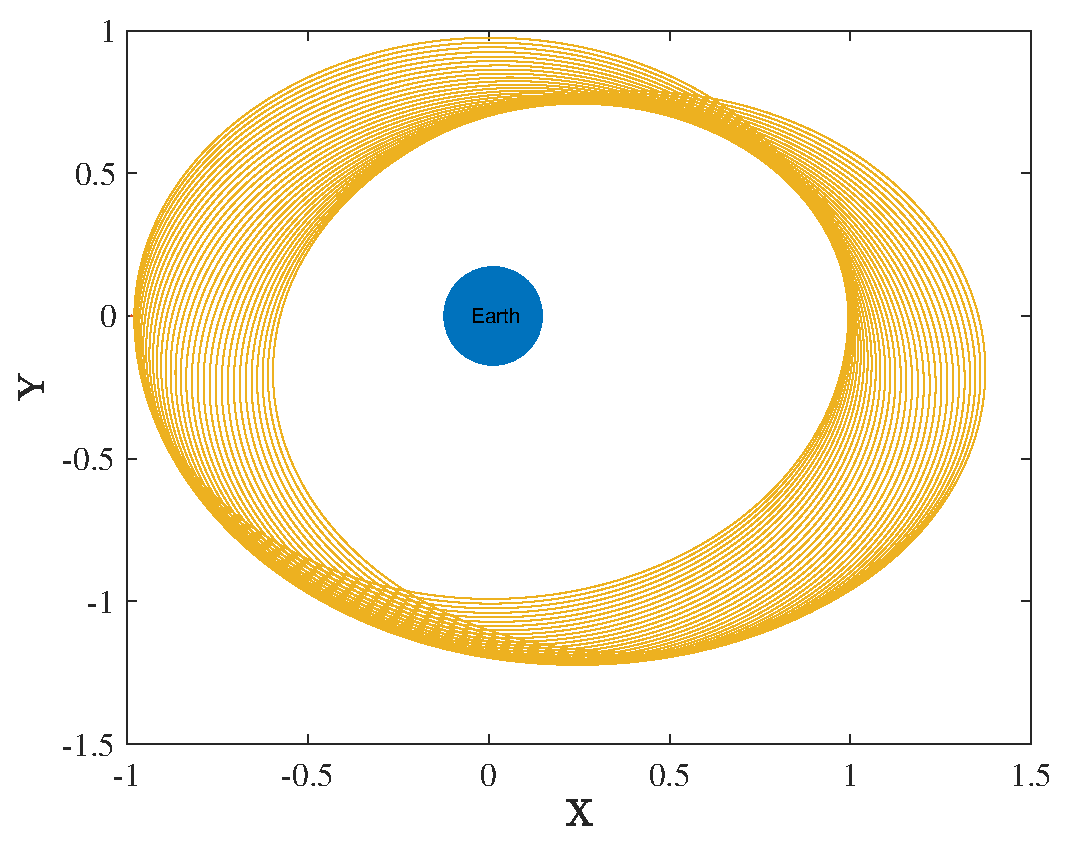
\includegraphics[width=12cm]{../Figure/Q4/xyplane}
\end{figure}